% ------------------------------------------------------------------------------
% ---------------------------------   CLASS    ---------------------------------
% ------------------------------------------------------------------------------
\documentclass[a4paper, 11pt]{article}

% ------------------------------------------------------------------------------
% ---------------------------------  COMMANDS  ---------------------------------
% ------------------------------------------------------------------------------
% -------------------------------    COMMANDS    -------------------------------
% ------------------------------------------------------------------------------
\usepackage{xspace} % para que anden los commands \snr, etc.

\newcommand{\tspace}{\bigskip}
\newcommand{\tamano}{\footnotesize}
\setcounter{secnumdepth}{4}
\setcounter{tocdepth}{4}

\newcommand{\reff}{\text{ref}\xspace}
\newcommand{\inn}{\text{in}\xspace}
\newcommand{\ter}{\text{th}}
\newcommand{\ntc}{\textsc{ntc}\xspace}
\newcommand{\ptc}{\textsc{ptc}\xspace}

\newcommand{\head}[1]{\textnormal{\textit{#1}}}

\usepackage{etoolbox}
\newcommand{\footnotetrucho}[2]{%
\ifstrempty{#2}{%
	\textsuperscript{\textit{#1}}%
	}{%
		\ifstrempty{#1}{%
			\scriptsize#2
		}{%
			\scriptsize\textsuperscript{\textit{#1}}\hspace{0.5em}#2
		}%
	}%
}%

% Para arreglar el espacio después de etc.
\makeatletter
\newcommand\etc{etc\@ifnextchar.{}{.\@}}
\makeatother

% ------------------------------------------------------------------------------

% ------------------------------------------------------------------------------
% ---------------------------------    USES    ---------------------------------
% ------------------------------------------------------------------------------
%\usepackage[margin=3cm]{geometry} % seteo los márgenes

\usepackage[T1]{fontenc} % para que use fuentes con caracteres especiales en el pdf y no los emule con a`, etc.

\usepackage[utf8]{inputenc} % para ingresar caracteres especiales (á, etc) directo en el .tex y no como \'a, etc.

%\usepackage{mathpazo} % mathpazo = palatino con math
\usepackage{lmodern}
	\normalfont\DeclareFontShape{T1}{lmr}{bx}{sc} { <-> ssub * cmr/bx/sc }{}
%\usepackage{libertine}
%\usepackage[libertine]{newtxmath}
%\usepackage{Alegreya}
%\usepackage[small,euler-digits]{eulervm}
%\usepackage{tgpagella}
%\usepackage[bitstream-charter]{mathdesign}

\usepackage[spanish]{babel}

\usepackage{csquotes} % Este debe ir inmediatamente después del babel

\usepackage[final]{microtype}

\usepackage{subfiles}

\pdfsuppresswarningpagegroup=1 % para que no moleste un warning	% paquetes varios
\usepackage{booktabs}

\usepackage{array}

\usepackage{multirow}

\usepackage{longtable}

\usepackage{pdflscape}

% ------------------------------------------------------------------------------
% Reglas un poco más gruesas
\let\oldtoprule\toprule
\renewcommand\toprule{\oldtoprule[1pt]}

\let\oldbottomrule\bottomrule
\renewcommand\bottomrule{\oldbottomrule[1pt]}
% ------------------------------------------------------------------------------	% paquetes para tablas
\usepackage{graphicx}

\usepackage[table]{xcolor}

\usepackage{float}
\usepackage{afterpage}
\usepackage{placeins}

\usepackage[%
	format			= plain,
	skip			= 0.5em,
	font			= footnotesize,
	labelfont		= sc,
	textfont		= bf,
	justification	= RaggedRight,
	labelsep		= newline,
	singlelinecheck	= off
]{caption}

\usepackage[%
	format			= plain,
	skip			= 0.5em,
	font			= footnotesize,
	labelfont		= bf,
	textfont		= bf,
	justification	= centering,
]{subcaption}

\usepackage{pstricks}

\usepackage{tikz}
	\usetikzlibrary{
		babel,
		patterns,
		shapes,
		arrows,
		shadows,
		backgrounds,
		decorations.markings,
		calc,
		fit
	}
\usepackage{circuitikz}

\usepackage{pgfplots}
	\pgfplotsset{compat=1.12}
%	\usepgfplotslibrary{
%		colorbrewer
%	}

\usepackage{pgfplotstable}	% paquetes para figuras
\usepackage{mathtools} %carga el amsmath y alguna cosa más

\usepackage{nicefrac}

\usepackage{steinmetz}	% para el argumento de los fasores

\usepackage{cancel}		% para cancelar términos

\usepackage{bm}

\usepackage{empheq}

\usepackage[mode=math,separate-uncertainty]{siunitx}
	\sisetup{%
		output-decimal-marker	= {,},
		list-final-separator	= { y },
		list-pair-separator		= { y },
		range-phrase			= { a },
	}

\usepackage{wasysym, amssymb, textcomp} % para usar los «Miscellaneous text symbols» de TexStudio

% ------------------------------------------------------------------------------
% Closed nth-root
\usepackage{letltxmacro}
\makeatletter
\let\oldr@@t\r@@t
\def\r@@t#1#2{%
\setbox0=\hbox{$\oldr@@t#1{#2\,}$}\dimen0=\ht0
\advance\dimen0-0.2\ht0
\setbox2=\hbox{\vrule height\ht0 depth -\dimen0}%
{\box0\lower0.4pt\box2}}
\LetLtxMacro{\oldsqrt}{\sqrt}
\renewcommand*{\sqrt}[2][\ ]{\oldsqrt[#1]{#2}}
\makeatother
% ------------------------------------------------------------------------------
% Los dos de abajo para que la coma del decimal quede más linda en modo math
\DeclareMathSymbol{,}{\mathord}{letters}{"3B}
\DeclareMathSymbol{\comma}{\mathpunct}{letters}{"3B}
% ------------------------------------------------------------------------------
% estas lineas arreglan el espacio alrededor de \left-\right
\let\originalleft\left
\let\originalright\right
\renewcommand{\left}{\mathopen{}\mathclose\bgroup\originalleft}
\renewcommand{\right}{\aftergroup\egroup\originalright}
% otra alternativa es usar \usepackage{mleftright} y cambiar los \left-\right por \mleft-\mright
% ------------------------------------------------------------------------------
% Un símil \hfill para el modo math
\makeatletter
\newcommand{\pushright}[1]{\ifmeasuring@#1\else\omit\hfill$\displaystyle#1$\fi\ignorespaces}
\newcommand{\pushleft}[1]{\ifmeasuring@#1\else\omit$\displaystyle#1$\hfill\fi\ignorespaces}
\makeatother
% ------------------------------------------------------------------------------	% paquetes para matemática
\usepackage{moresize} % para usar el HUGE

\usepackage{datetime} % para poner la hora

\usepackage[textsize=scriptsize]{todonotes} \setlength{\marginparwidth}{2cm}

\usepackage[nottoc,numbib]{tocbibind}

\usepackage{enumitem}

\usepackage{relsize}

\usepackage{pdfpages}

\usepackage[
	bookmarks,
	bookmarksopen,
	bookmarksnumbered,
	hidelinks
]{hyperref}
% ------------------------------------------------------------------------------
% Para arreglar el espacio en las notas al pie.
\let\oldfootnote\footnote
\renewcommand\footnote[1]{\oldfootnote{\hspace{0.5em}#1}}

\let\oldfootnotetext\footnotetext
\renewcommand\footnotetext[1]{\oldfootnotetext{\hspace{0.5em}#1}}
% ------------------------------------------------------------------------------
% To prevent a page break before an itemize list
% http://tex.stackexchange.com/questions/2644/how-to-prevent-a-page-break-before-an-itemize-list
\makeatletter 
\newcommand\mynobreakpar{\par\nobreak\@afterheading} 
\makeatother
% ------------------------------------------------------------------------------	% Varios

\title{\huge Resumen de Papers\\}
\author{\textsc{Alejandro Goday}}
%\date{23 de junio de 2015}

\graphicspath{{img/}}
% ------------------------------------------------------------------------------
% -------------------------------    DOCUMENT    -------------------------------
% ------------------------------------------------------------------------------
\begin{document}
	
	\pagenumbering{arabic}
	\maketitle
%	\tableofcontents

\section{Evaluation of measurements of the conductivity of quarter milk samples for	the early diagnosis of mastitis}
\subsection{Materiales y Métodos}
Se recolectó datos de un 31 vacas en el sudeste de Inglaterra durante 15 semanas. Las vacas fueron ordeñadas con una unidad que medía y registraba los valores de conductividad de muestras individuales de leche de cuartos. La conductividad era reportada para cada cuarto en términos del aumento en porcentaje respecto a la conductividad promedio de las medidas de los 14 días previos, una vez que este exceso pasaba un cierto umbral del 10 \% o a veces 15 \%. A los excesos por encima de estos umbrales se les llama \emph{triggers}.  

\subsection{Conteo de células somáticas}
Se recolectó muestras individuales de cada cuarto de cada vaca una vez a la semana, a fines de determinar el conteo de células somáticas.

\subsection{Análisis de datos}
\begin{itemize}
	\item Se analizó el conteo de células somáticas de cada muestra de leche de cada cuarto
	\item Los datos fueron tratados como para dar promedios semanales, resultando en un máximo de 465 semanas-vaca de datos para valores correspondientes a la vaca entera, y un máximo de hasta 1600 semanas-cuarto de datos para valores correspondientes a cuartos individuales.
	\item Se analizó los datos en períodos de una semana, primero usando datos de tres días antes y tres días después del día de conteo de células somáticas y luego examinando los datos de los 7 días antes de la realización del conteo de células somáticas.
\end{itemize}
\subsection{Ocurrencia de \emph{triggers}}
Durante el período de registro, sólo 194 semanas-vaca (42 por ciento del total de semanas vaca) tuvieron uno o más \emph{triggers} de conductividad por cuartos con umbral 10 \%. La tabla \ref{fig:semanasvaca} muestra los números de semanas-vaca en los cuales ocurrieron \emph{triggers} en la conductvidad en uno, o dos o tres o cuatro cuartos de una vaca.
\begin{figure}[H]
	\centering
	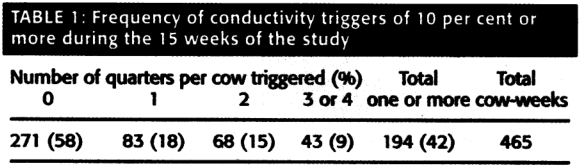
\includegraphics[width=1.0\linewidth]{img/Table1}
	\caption{Tabla de semanas vaca en las que ocurrieron \emph{triggers} en la conductividad \label{fig:semanasvaca}}
\end{figure}

En términos de cuartos, 310 semanas-cuarto (20 porciento del total) tuvieron un \emph{trigger} de conductividad con umbral 10\%. Si se incrementaba el umbral a 15\%, menos del 14\% de las semanas-cuarto tenían un \emph{trigger}.

\subsection{\emph{Triggers} y conteo de Células Somáticas}
\begin{itemize}
	\item La media geométrica del conteo de células somáticas fue significativamente más alta en semanas-cuarto con \emph{Triggers}, que en semanas-cuarto sin \emph{Triggers}
	\item La media geométrica del conteo de células somáticas fue significativamente más alta en semanas-cuarto con un mayor incremento en la conductividad.
	\item Dicha media tuvo sus valores más bajos en semanas sin \emph{Triggers} pero incrementaba a medida que el porcentaje incrementaba desde el 10\% al 20 \% (véase figura \ref{fig:Geomean} ).
	\item Los números por encima de cada barra del histograma indican la cantidad de semanas-cuarto en cada categoría.
\end{itemize}
\begin{figure}[H]
	\centering
	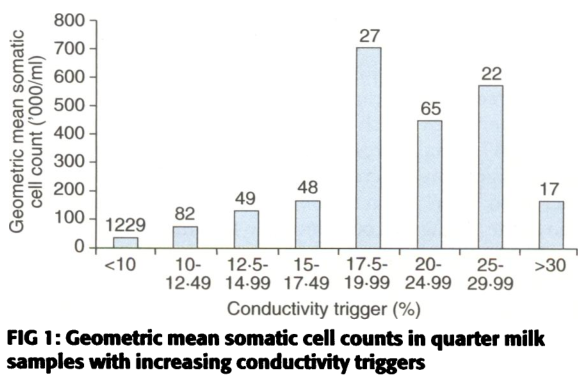
\includegraphics[width=0.7\linewidth]{img/Geomean}
	\caption{Media geométrica de conteos de células somáticas en muestras de leche de cuartos a medida que aumentan los umbrales de los \emph{Triggers}  \label{fig:Geomean}}
\end{figure}
\subsection{Estimación de Sensibilidad y Especificidad}
Sea $SCC$ el conteo de células somáticas. La semana-cuarto se puede categorizar como:
\begin{itemize}
	\item No infectada si $SCC < 200.000$ células/ml
	\item Infectada si $SCC \geq 200.000$ células/ml 
\end{itemize}
Estas categorías están relacionadas con las semanas-cuartos en las que hubo \emph{Triggers} de 10 \% o más. Los resultados para \emph{triggers} de conductividad registrados 3 días antes y tres días después de la realización del conteo de células somáticas, se presentan en la figura \ref{fig:table2}.
\begin{figure}[H]
	\centering
	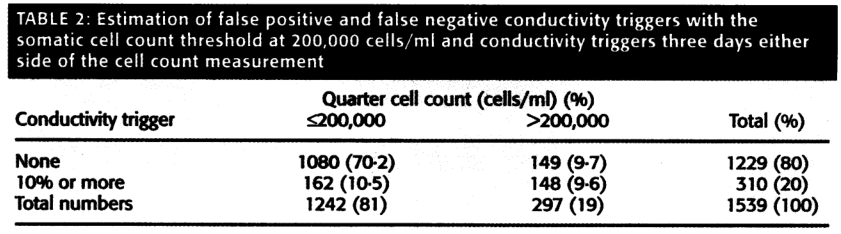
\includegraphics[width=0.9\linewidth]{img/table2}
	\caption{ \label{fig:table2}}
\end{figure}
En base a esto se clasificaron a las semanas-cuarto en FP, FN, TP Y TN.
\begin{itemize}
	\item Cuando no hay trigger y está infectada: $FN<10\%$ 
	\item Cuando hay trigger y no está infectada: $FP=10$
\end{itemize}
De los datos se obtuvo:
$$\text{Sensibilidad}=\frac{TP\times 100}{TP+FN}=\frac{148\times 100}{148+149}=50\% $$
$$\text{Especificidad}=\frac{TN\times 100}{TN+FP}=\frac{1080\times 100}{1080+162}=87\% $$

Los valores predictivos negativos y positivos son los siguientes:
$$\text{VPP}=\frac{TP\times 100}{TP+FP}=\frac{148\times 100}{148+162}=48\% $$

$$\text{VPN}=\frac{TN\times 100}{TN+FN}=\frac{1080\times 100}{1080+149}=88\% $$

Tomando los valores de conductividad en los 7 días previos, la sensibilidad bajó a 46\% y la especificidad quedó en 87 \%. El VPP se redujo a 45\% y el VPN bajó a 87\%.
\subsection{En conclusión}
\begin{itemize}
	\item La conductividad de la leche puede variar considerablemente en ausencia de mastitis debido a factores como la etapa de lactancia, el intervalo de ordeñe y el celo. Estos factores complican la interpretación de cambios en la conductividad y la precisa selección de vacas para una terapia antibiótica temprana.
	\item Hay una relación significativa entre la conductividad de la leche de cada cuarto, y el incremento de células somáticas.
	\item Una relación significativa no es condición suficiente para una prueba útil. La prueba tiene que tener valor predictivo, con sensibilidad y especificidad suficientemente altas para que se pueda hacer predicciones útiles.
	\item Los resultados sugieren que la conductividad de muestras individuales de cuartos no es adecuada para ser utilizada como predictor temprano de mastitis, por dos razones. \\\\
	La sensibilidad es demasiado baja, con una proporción muy alta de casos no siendo identificados los suficientemente temprano, esto es, antes de un incremento en el conteo de células somáticas. Sin embargo, la sensibilidad pobre no haría por sí sola que la prueba fuera inútil, porque la detección temprana y el tratamiento del 50\% de las vacas en riesgo podrían ser significativamente beneficiosos. 
	\item Es la proporción de falsos positivos, lo que excluye la posibilidad de usar únicamente la conductividad de la leche de cada cuarto.
	\item El Valor Predictivo Positivo fue cercano al 50\%. Por tanto, si la conductividad de la leche de cada cuarto fuera utilizada para identificar vacas a someter a un tratamiento temprano, esto resultaría en un porcentaje inaceptable de tratamientos injustificados, porque casi tantas vacas serían tratadas innecesariamente como las que recibirían tratamiento temprano.
	\end{itemize}



%\subsection{¿Cuál es el mínimo ángulo que puede resolver el ojo humano?}
%La agudeza visual se mide como el angulo abarcado por el detalle visible más pequeño en un objeto. Al diseñar sistemas de televisión se toma como referencia una agudeza visual del del orden de 1 minuto de arco. Denotando dicho ángulo como $\alpha$, tenemos que $\alpha=2.91\times 10^{-4}\textbf{radianes}$. La figura \ref{fig:visualAcuity} ilustra el concepto de agudeza visual.
%\begin{figure}[H]
%	\centering
%	\includegraphics[width=1.0\linewidth]{img/visualAcuity}
%	\caption{Agudeza Visual \label{fig:visualAcuity}}
%\end{figure}
%\subsection{¿Cuál es la relación ($\nicefrac{D}{H}$) para televisión en definición estándar? De acuerdo a esto, enuncie cuáles son las normas analógicas que todavía se usan, en cuanto a cantidad de líneas y frecuencia de cuadro.}
%El grado al cual un medio visual como la televisión puede reproducir detalles finos se expresa en términos de resolución. La resolución en televisión es igual al número de líneas alternadamente blancas y negras que pueden ser resueltas verticalmente sobre toda la altura de la pantalla. Se expresa en cantidad de líneas por altura de la imagen (LPH). Los estándares de 525 y 625 líneas fueron desarrollados tomando en consideración la \emph{agudeza visual} del ojo y asumiendo condiciones de visión típicas en una casa promedio. Refiriéndonos a la figura \ref{fig:visualAcuity}, en definición estándar esto se traduce en:
%\[\alpha=2.91\times 10^{-4}radianes\]
%\[\frac{D}{H} = 6\]
%
%Donde:
%	\begin{itemize}
%		\item $H$ es la altura de la imagen
%		\item $D$ es la distancia de visionado
%		\item $\alpha$ es el mínimo ángulo que el ojo puede resolver
%	\end{itemize}
%En base a los números previamente mencionados se obtiene el número $N_v$ de elementos en la vertical que el ojo puede resolver como:
%
%$$N_v=\frac{H}{\alpha D}=\frac{1}{6\times 2.91\times 10^{-4}}\simeq 527\hspace{0.1cm} \textbf{líneas}$$
%
%Esto da origen a las cantidades de líneas de los dos sistemas de televisión convencionales. Dichos sistemas son:
%	\begin{itemize}
%		\item 525 líneas / 60 Hz de frecuencia de campo (Que la frecuencia de campo sea 60Hz es lo mismo que decir que la frecuencia de cuadro es 30fps)
%		\item 625 líneas /50Hz de frecuencia de campo (Que la frecuencia de campo sea 50Hz es lo mismo que decir que la frecuencia de cuadro es 25fps)
%	\end{itemize}
%
%\section{Barrido entrelazado}
%\subsection {¿En qué consiste y cómo se consigue? (Robin y Poulin 1.3.1 The Scanning Process)}
%Los estándares convencionales de televisión reflejan la tecnología de pickup and display de los años treinta. Esto asume que la cámara usa un \emph{pickup tube} donde la imagen se concentra sobre una capa fotoconductora. Cargas eléctricas, proporcionales a la escena iluminada en cada punto, son reveladas y almacenadas capacitivamente en esta capa.\\\\
%Un rayo de electrones es utilizado para convertir la imagen de carga en una corriente eléctrica. Este rayo es desviado continuamente sobre la imagen en dos campos consecutivos de líneas horizontales. Cada campo contiene la mitad del total del número de líneas en las cuáles la imagen es barrida. Dos campos consecutivos (campo 1 y campo 2) son desplazados verticalmente de tal forma que sus líneas de barrido son entrelazadas y juntas forman un cuadro (\emph{frame}). \\\\
%La imagen es barrida  de izquierda a derecha, comenzando desde arriba y trazando sucesivas líneas hasta que se alcanza el fondo de la misma. El rayo luego vuelve hacia arriba  y el proceso se repite. La desviación continua del rayo de electrones se logra sometiéndolo a dos campos magnéticos perpendiculares (vertical y horizontal) que resultan del flujo de repetitivas corrientes con forma de diente de sierra a través de espiras de deflexión. La tasa de repetición de la componente horizontal se relaciona con la componente vertical mediante un factor n, resultando en la formación de n líneas durante un período vertical completo.\\\\
%Los tiempos de vuelta del rayo no son utilizados para la transmisión de la señal de video sino que son utilizados para la transmisión de información auxiliar como por ejemplo información de sincronización  de los barridos vertical y horizontal.\\\\
%En dispositivos de visualización, un tubo de rayos catódicos (CRT) recrea la imagen original. Un rayo de electrones enfocado, desviado horizontalmente y verticalmente en sincronía con el rayo de electrones del pickup tube, se proyecta sobre una pantalla de visualización recubierta en fósforo. La corriente del rayo del CRT es, idealmente, proporcional a la corriente del rayo del pickup tube y, las corrientes de deflexión que pasan a través de sus espiras de deflexión están en sincronía con las del pickup tube. En la realidad, la corriente del rayo de electrones del CRT no tiene una relación lineal con la tensión de la señal eléctrica. Para corregir esto, el amplificador de video de la cámara introduce una no linealidad opuesta, llamada “corrección gamma”, resultando en una relación lineal entre el brillo original de la imagen y el brillo reproducido por el CRT.
%
%\subsection{En la época de la TV en blanco y negro: ¿Por qué se hizo coincidir la frecuencia de campo, con la frecuencia de la red de energía eléctrica? ¿Qué se buscó con esto?}
%
%Porque bajo condiciones extremas,{ \bf un display en sincronía con la frecuencia de la red, reduce la visibilidad de distorsiones en el barrido causadas por campos magnéticos interferentes y componentes armónicas, en caso de que existan}. Esta visibilidad reducida es obtenida cuando el receptor y el transmisor operan con la misma fuente de potencia, que no siempre es el caso. En consecuencia, la práctica de sincronizar la tasa de campo con la frecuencia de la red eléctrica ha sido discontinuada y hoy, la frecuencia de barrido vertical es sólo nominalmente igual a la frecuencia de la red, dado que es obtenida contado regresivamente desde un oscilador de alta frecuencia controlado por cristal, que es altamente estable.
%
%
%
%\section{Modulación de video y canal de transmisión}
%	\subsection{¿Con qué tipo de modulación se realiza la transmisión analógica de video?¿Cuál es el ancho de banda de transmisión?}
%Dado un ancho de banda de video específico en banda base, por ejemplo $4.2$MHz en estándar de barrido 525/60, la modulación en amplitud convencional de la portadora de video resulta en bandas laterales superior e inferior conteniendo información idéntica. El ancho de banda transmitido en este caso resulta ser el doble del ancho de banda en banda base. Para el estándar 525/60 esto requeriría un ancho de banda transmitido de $8.4$MHz para la información de video. El estándar 625/50 requeriría como mínimo $10$ MHz de ancho de banda transmitido para la información de video. A estas cifras se le debe agregar por otro lado el espectro requerido por la portadora de audio y sus bandas laterales.\\\\
%Preocupaciones conservadoras en términos de espectro y de asignación de frecuencias han llevado a varios países a especificar un ancho de banda de canal de transmisión reducido:
%
%\begin{itemize}
%	\item {\bf En países 525/60 el ancho de banda especificado de canal de transmisión es de $6$ MHz}.
%	\item {\bf En países 625/50 el ancho de banda especificado de canal de transmisión es de $7$ u $8$ MHz}.
%\end{itemize}
%
%El método empleado para asignar un ancho de banda de transmisión reducido, a partir del ancho de banda de video en banda base consiste en:
%
%\begin{itemize}
%	\item {\bf Transmitir todo el ancho de la banda lateral superior}.
%	\item {\bf Transmitir la banda lateral inferior con ancho de banda reducido }.
%\end{itemize}
%
%{\bf Para lograr esto se utiliza un filtro en el transmisor que elimina la porción de la banda lateral inferior correspondiente a las altas frecuencias. A este método se le denomina \emph{Transmisión de Banda Lateral Vestigial Inferior (Vestigial Lower Sideband Transmission)}}
%
%\newpage
%La figura \ref{fig:vsb} muestra en detalle la estructura de canal correspondiente al estándar CCIR M utilizado en Norteamérica para señales monocromáticas. Se destacan las siguientes características:
%
%\begin{itemize}
%	\item El ancho de banda es 6MHz
%	\item La portadora de video está situada 1.25MHz por encima del extremo inferior del canal de transmisión
%    \item Se envían los $4.2$ MHz de la banda lateral superior de video.
%    \item Se envía una banda lateral reducida (vestigial)  de $0.75$ MHz
%    \item Se envía además en el mismo canal, una portadora de audio modulada en frecuencia con una frecuencia central $4.5$ MHz por encima de la frecuencia de la portadora de video.
%\end{itemize}
%
%
%\begin{figure}[H]
%	\centering
%	\includegraphics[width=1.0\linewidth]{img/vsb}
%	\caption{Canal de transmisión y espectro de señal monocromática para Banda Lateral Vestigial Inferior en CCIR M. \label{fig:vsb}}
%\end{figure}
%
%
%
%%El tipo de modulación empleada en la transmisión analógica de video es    Banda Lateral Vestigial. Lo que hace esta modulación es mover a una cierta frecuencia una de las bandas laterales junto con vestigios de las bajas frecuencias de la otra banda.
%
%%\subsection{¿Cuál es el ancho de banda de transmisión?} 
%%El ancho de banda de transmisión de video es 6MHz para 525/60 y 7 u 8MHz para 625/50.
%\subsection{¿Cuáles son las ventajas de la modulación negativa de video?}
%En un sistema de modulación negativa, al incrementarse el brillo, decrece la amplitud de la envolvente de modulación, lo contrario a lo que ocurre en el sistema de envolvente positiva. 
%Las ventajas son:
%\begin{itemize}
%  \item Los pulsos de ruido en la señal transmitida habrán de incrementar la amplitud de la portadora y se moverá más hacia el negro.
%
%  \item La amplitud de la portadora permanecerá baja la mayor parte del tiempo dado que la señal es más blanca que negra, entonces {\bf se ahorra en potencia de transmisión}.
%\end{itemize}
%
%\section{¿Cuáles fueron las pautas que se debieron cumplir para adoptar la norma analógica de transmisión de señales en color?}
%
%Lo principal a considerar en el desarrollo de los estándares importantes de televisión a color (NTSC, PAL, SECAM) fue la compatibilidad con el estándar existente de televisión monocromática. Hay varios aspectos a tener en cuenta, que son:
%
%\begin{itemize}
%	
%\item Compatibilidad con blanco y negro: Un receptor monocromático debe poder reproducir correctamente en blanco y negro el contenido de brillo de una señal a color sin interferencia visible de la información de color.
%
%\item Compatibilidad inversa (Reverse compatibility): Un receptor de color debe reproducir una señal monocromática correctamente en tonos de gris sin componentes espurias de color.
%
%\item Compatibilidad de barrido (Scanning Compatibility): El sistema de barrido utilizado para transmisiones de color debe ser idéntico a aquel utilizado para el servicio monocromático existente.
%
%\item Compatibilidad de canal (Channel Compatibility): El sistema color debe caber en el canal de televisión monocromática existente y utilizar el mismo espaciado entre las portadoras de visión y sonido.
%
%\end{itemize}
%\newpage
%\section{De acuerdo a la forma que tiene el espectro de la señal de blanco y negro (luminancia) explique cómo se consigue introducir la información de color, dentro del mismo ancho de banda de la señal de luminancia, para poder formar el video compuesto de color y transmitirlo.(Robin y Poulin 1.6 - The Spectrum of the Video Signal y 2.2.2 - The NTSC system)}
%Las componentes frecuenciales de una imagen ocupan una banda de frecuencia amplia. Sin embargo, el espectro no es continuo. Las componentes espectrales están espaciadas en intervalos, como puede apreciarse en la figura~\ref{fig:espectroPeine}. Dicha figura representa el espectro de una imagen estacionaria para el estándar de barrido 525/60.
%
%\begin{figure}[H]
%	\centering
%	\includegraphics[width=1.0\linewidth]{img/monospec}
%	\caption{Espectro de una escena estacionaria de video monocromático para el estándar 525/60. \label{fig:espectroPeine}}
%\end{figure}
%
%Hay una fuerte componente en la frecuencia de barrido horizontal $f_H$ y componentes en múltiplos de dicha frecuencia. También hay una fuerte componente en la frecuencia de barrido vertical(repetición de campo) $f_V$ y componentes en múltiplos de $f_V$. El estandar de barrido 625/50 tiene un espectro similar, excepto que con $f_H=15625$Hz y $f_V=50Hz $.\\\\
%En caso de haber detalles que cambien de un cuadro al siguiente, existirá además una componente en la frecuencia de cuadro ($30$ o $25$ Hz).\\\\
%Las componentes en la frecuencia de barrido horizontal y sus múltiplos tiene bandas laterales en las frecuencias de campo y de cuadro, y múltiplos de éstas.\\\\
%Finalmente, hay una fuerte componente a frecuencia cero que representa al brillo promedio de la imagen. Si la imagen contiene movimiento, el espectro se vuelve más complejo debido a la adición de más componentes. En teoría el espectro se extiende hacia infinito, pero es limitado en banda a la frecuencia máxima de modulación de video especificada por el estándar de transmisión en efecto.\\\\
%Las señales diferencias de color se multiplexan en frecuencia con la de luminancia de forma tal que se transmiten en
%los «agujeros» que hay en el espectro de la señal luminancia. Para esto las señales $(R-Y)$ y $(B-Y)$ modulan en fase y cuadratura respectivamente, una portadora de frecuencia $f_{sc}=\frac{\textbf{Impar}}{2} \times f_H$, que para $\textbf{Impar}= 455$ vale aproximadamente $3.58$ MHz.
%Las señales diferencia son moduladas en transmisión con un ancho de banda de $600$ kHz(debido a restricciones de ancho de banda) y en estudios con un ancho de banda de $1.3$MHz. En la figura \ref{fig:colorVsb} se puede ver el espectro de las señales enviadas en un canal de transmisión para un sistema color NTSC.
%
%\begin{figure}[H]
%	\centering
%	\includegraphics[width=1.0\linewidth]{img/colorVsb}
%	\caption{Espectro de señales transmitidas en un canal de televisión color para 525/60. \label{fig:colorVsb}}
%\end{figure}
%\newpage
%\section{Dibuje un diagrama de bloques con el codificador NTSC y explique su funcionamiento(Robin y Poulin- 2.2.2)}
%
%En la figura \ref{fig:Codificador NTSC} se muestra el diagrama de bloques de un codificador NTSC.
%
%\begin{figure}[H]
%	\centering
%	\includegraphics[width=1.0\linewidth]{img/CodificadorNTSC}
%	\caption{Diagrama de bloques simplificado de un codificador NTSC B-Y/R-Y \label{fig:Codificador NTSC}}
%\end{figure}
%
%Se alimenta con señales de verde, azul y rojo a una matriz resistiva que combina algebraicamente porcentajes de estas
%señales de colores primarios para formar la señal de luminancia y las dos señales de diferencia de color. Las señales de diferencia de color son limitadas en banda antes de ser introducidas en sus respectivos moduladores balanceados. Una subportadora de $3.58$ MHz alimenta al modulador de $B-Y$ y, a través de una red de corrimiento de fase de 90°  alimenta al modulador de $R-Y$.\\\\
%Se retarda la señal $Y$ para compensar el retardo en la croma
%introducido por los LPF  por los que pasan las señales de
%diferencia de color. Además se envían 9 ciclos de una portadora (burst) desfasada 180° durante el \emph{backporch} del intervalo de \emph{horizontal blanking}, que sirve para que el receptor tenga una referencia de donde se encuentra la fase de 180° del transmisor y de su frecuencia, y de esa forma, pueda sintonizarse con él.  El sumador combina la luminancia, las bandas laterales de croma, composite sync, y la portadora con desfasaje de 180° (burst) en una señal color compuesta.
%
%\section{Dibuje un diagrama de bloques con el codificador PAL y explique su funcionamiento.(Robin y Poulin Capítulo 2 - Páginas 67-70)}
%
%En la figura \ref{fig:Codificador PAL} se muestra el diagrama de bloques del codificador PAL.
%\begin{figure}[H]
%	\centering
%	\includegraphics[width=1.0\linewidth]{img/codificadorPAL}
%	\caption{Diagrama de bloques simplificado de un codificador PAL \label{fig:Codificador PAL}}
%\end{figure}
%
%Una vez realizadas las respectivas correcciones gamma, las señales verde, azul y rojo son introducidas a una matriz que produce la señal de lumniancia (Y) y las dos señales de diferencias de color ($U$ y $V$ serían las señales $(B-Y)$ y $(R-Y)$ ).
%Cada una de las señales de diferencia de color es limitada en ancho de banda a $1.2$ MHz antes de introducirlas a sus respectivos moduladores balanceados. Una subportadora de $4.43$ MHz alimenta al Modulador $U$ directamente y al Modulador $V$ a través de una red de corrimiento de fase de $\pm 90$° (en valor absoluto). Se genera también una subportadora de $\pm 135$ phased-switched gated . El alternado de fase de las supbortadoras de V (en el libro decía U pero para mí estaba mal) y burst ocurre a una frecuencia de $\nicefrac{f_H}{2}=7812.5$ Hz. Se retarda la señal de luminancia (Y)  para compensar el retraso de croma introducido por los filtros pasabajos utilizados para limitar en banda las señales de diferencia de color. El sumador combina la luminancia, las bandas laterales de croma, el composite sync y el gated subcarrier burst en una señal compuesta de color (color composite signal).
%
%\section{¿Cuál es la diferencia que introduce el sistema PAL respecto del NTSC? Justifique por qué se introdujo PAL.}
%La diferencia principal entre los sistemas de televisión color NTSC y PAL radica en que en PAL la fase de la subportadora de (R-Y) se invierte entre líneas consecutivas.\\\\ La razón principal por la cual se introdujo el sistema PAL de televisión color fue para superar algunas deficiencias en los equipos de estudio y de transmisión. {\bf Uno de los principales defectos de los sistemas de televisión color NTSC es su sensibilidad a distorsiones no lineales que resultan en fases diferenciales. El proceso PAL transforma la fase diferencial (que tendría como consecuencias cambios del tinte de los colores) en ganancia diferencial, logrando como resultado cambios en la saturación del color que son menos notorios}.
%
%\section{En la norma ITU-R 601, ¿qué señales son digitalizadas? ¿qué frecuencia de muestreo se utiliza y por qué se la seleccionó?}
%
%Las señales digitalizadas son la de luminancia ($Y$) y las de diferencia de color (escaladas de tal forma que no presenten una excursión excesiva).\\\\ La frecuencia de muestreo utilizada para muestrear la señal de luminancia es de $13,5$ MHz, mientras que las señales de diferencia de color se muestrean a  $6,75$MHz(o sea, la mitad de la frecuencia de muestreo de luminancia). Se eligió la mitad para no enviar una cantidad excesiva de bits y de esta forma requerir un ancho de banda de transmisión tan alto.\\\\
%La frecuencia de muestreo de luminancia de 13,5 MHz fue seleccionada para permitir un número entero de períodos de muestreo en los intervalos de línea, tanto del estándar 525/60 como de 625/50, obteniéndose de esta forma lo que se conoce como \emph{muestreo ortogonal}, en el cual, las muestras de las distintas líneas quedan alineadas verticalmente. Un ejemplo de esto último se muestra en la figura~\ref{fig:422}. Otro requisito necesario para la frecuencia de muestreo elegida es cumplir la hipótesis del teorema de muestreo. Es por esta razón que se descarta la idea de muestrear $2.25$MHz, que en principio, si bien parecería permitir que quepan una cantidad entera de muestras en un intervalo de línea, que no es mayor al doble de ancho de banda ($12$MHz).
%
%\begin{figure}[H]
%	\centering
%	\includegraphics[width=1.0\linewidth]{img/422sampling}
%	\caption{Estructura de muestreo 4:2:2 para 525/60 \label{fig:422}}
%\end{figure}
%
%La frecuencia de muestreo de luminancia se obtiene del sincronismo de video de entrada usando un oscilador PLL que opera a $858 \times f_H$ en el standard 525/60 y $864\times f_H$ en el estándar 625/50.
%\newpage
%\section{Dibuje un diagrama de bloques del equipo que realiza la distribución de la señal serie de video digital, explicando sus componentes. (Robin y Poulin - Capítulo 7)}
%
%La figura \ref{fig:bitSerial} muestra el diagrama en bloques de la distribución en forma digital serie.
%\begin{figure}[H]
%	\centering
%	\includegraphics[width=1.0\linewidth]{img/bitSerial}
%	\caption{Modelo de distribución de video Bit-serial \label{fig:bitSerial}}
%\end{figure}
%\begin{itemize}
%\item  {\bf Source Encoder}: Es un convertidor convencional analógico/digital.
%
%\item {\bf Channel Encoder:} transforma la señal de salida digital bit-parallel del convertidor A/D en una señal digital bit-serial, adecuada para enviar por el medio elegido (por ejemplo, un cable coaxil). La señal puede ser afectada por el ruido térmico en la etapa de entrada del receptor.
%\item {\bf Receiver Channel Decoder:} Deserializa la señal digital bit-serial recibida y recupera la señal de video digital
%bit-parallel.- Un excesivo ruido térmico puede afectar al \emph{receiver channel decoder}, resultando en errores en los bits o pérdidas totales de los mismos.
%\item {\bf Signal Decoder:} es un convertidor convencional digital/analógico, que recupera la señal de video análogica original.
%\end{itemize}
%La bit-serial data rate esta dada por:
%$$\textbf{Bit-serial rate (Mbps)} = \textbf{Parallel bit rate} \left( \frac{Mpalabras}{s} \right)\cdot \frac{\textbf{cantidad de bits}}{palabra} $$
%La digital bit-serial rate en el sistema 4:2:2 es igual a:    $$\textbf{Bit-serial rate} =  \frac{27 \textbf{Mpalabras}}{s} \cdot \frac{10 \textbf{bits} }{\textbf{palabra}} = 270 Mbps$$
%\section{Explicar en qué consiste la señal de referencia temporal (SAV y EAV) en ITU-R 601}
%Dos señales de referencia temporal se multiplexan en el “stream” de datos, inmediatamente antes y después de la línea digital activa SAV(Start of Active Video) y EAV(End of Active Video).  Cada señal consta de 4 palabras:
%\begin{center}
%	$\displaystyle{3FF}$ $\displaystyle{000}$ $\displaystyle{000}$ $\displaystyle{XYZ}$
%\end{center}
%
%
% Las primeras 3 palabras son fijas, reservadas para identificación temporal. Identifican el comienzo de la información de sincronismo SAV y EAV.
%Por otro lado:
%\begin{itemize}
%\item XYZ es una palabra variable de la forma:\\
% 	$\bullet$ $1$ $F$ $V$ $H$ $P_3$ $P_2$ $P_1$ $P_0$ $1$ $0$
%\item F identificación de campo\\
%	 $\bullet$ F=0 campo 1\\ 
%	 $\bullet$ F=1 campo 2
%
%\item V identificación de borrado vertical\\
%	$\bullet$ V=0 video activo\\  
%	$\bullet$V=1 borrado vertical
%
%\item H identificación de borrado horizontal\\
%    $\bullet$ H=0 para SAV \\
%    $\bullet$ H=1 para EAV
%
%\item $P_3 P_2 P_1 P_0$  son para corrección de errores simples y detección de errores dobles en  $FVH$
%\end{itemize}
%
%\section{Explicar el siguiente diagrama de bloques, en su conjunto y analizando el rol de cada uno de sus componentes, y dar los valores para A, B y C:}
%\begin{figure}[H]
%	\centering
%	\includegraphics[width=1.0\linewidth]{img/cod422}
%	\caption{Codificador 4:2:2 \label{fig:cod422}}
%\end{figure}
%.\\
%$A=13.5MW/s$\\ 
%$B = 6.75MW/s$\\
%$C= 27MW/s$\\
%La figura  muestra un diagrama en bloques simplificado de un codificador 4:2:2 con salida “bit-parallel” multiplexada en el tiempo a 27 Mwords/seg.- La información digital Y va a una rate de 13,5 Mwords/seg ( duración de la muestra en 74 nseg ) y Cb y Cr en información digital a una “data rate” de 6,75 Mwords/seg ( duración de la muestra 148 nseg ) y todo esto se alimenta a un combinador de data digital que lee secuencialmente la  data digital a una “data rate” de 27 Mwords/seg ( duración de la muestra de 37 nseg ).- En este diagrama la numeración de las muestras parten con 1 en vez de 0, para mostrar que las muestras Cb y Cr están juntas con las muestras
%“odd” ( 1; 3; 5;......) Y.- Las sentencias de video son enviadas con la velocidad de 27 Mwords/seg multiplexadas, y transmitidas en el siguiente orden: Cb; Y; Cr; Y; Cb; etc., donde las primeras 3 palabras ( Cb, Y y Cr ) se refiere a la luminancia “odd” y las muestras diferencia color y la siguiente palabra Y se refiere a la muestra donde Y esta sola.- La primera palabra de data de video de cada línea activa es Cb.
%\section{Explicar cómo son las estructuras de muestreo 4:2:2, 4:1:1 y 4:2:0. ¿Qué las diferencia?¿Cuál de ellas ofrece mayor resolución? ¿Por qué existen las otras? }
\end{document}


